\documentclass[output=paper]{langsci/langscibook}
\author{Koenraad Kuiper\affiliation{University of Canterbury, New Zealand}}
\title{Multiword expressions and the Law of Exceptions}

\abstract{This chapter proposes the existence of a linguistic universal, the \is{Law of Exceptions} Law of Exceptions. It hypothesizes that a relationship exists between the grammar of a language and its lexicon such that all regularities expressed in the grammar of a language are matched by exceptions which are manifested in the lexicon of that language. It is also proposed that lexical idiosyncrasies are of two types. Type~1 idiosyncrasies are in the nature of arbitrary restrictions on options provided in the grammar while Type~2 idiosyncrasies involve breaches of the rules of the grammar. To test this law requires an initial examination of the linguistic domains where it might be tested. As a preliminary step to testing these ideas, this chapter is scoping exercise looking chiefly at the structural properties of a subset of multiword expressions (MWE). It shows, following \citet{Barkema1996}, that many properties of MWEs cross-classify. The aim of the overview is then to examine domains of the \is{morphosyntax} morphosyntax of any language which might be analysed for sources of structural idiosyncrasy and thus to determine how individual languages might vary in this respect. Languages of exemplification are \il{English} English, which has a relatively fixed word order and slight inflectional system, and, to a lesser extent Dutch and M\=aori, an Oceanic language.}

\maketitle

\begin{document}

\section{Introduction}

In the traditional grammar-lexicon model of human linguistic knowledge, the grammar accounts for the regularities in the language which a native speaker is taken to have acquired and thus the predictabilities in its sentences. The lexicon has traditionally been ‘an appendix of the grammar, a list of basic irregularities,’ \citep[274]{Bloomfield1933}. While this distinction is increasingly contested, it will be maintained here. It is, in any case, an open question as to just where the boundary between the grammar and the lexicon lies and, more significantly for what follows, what kinds of ‘basic irregularities’ are possible; that is to say what kinds of idiosyncrasies can be expected to occur in the lexical items of a language. 

Bloomfield’s characterisation raises the question as to the kinds of basic irregularities which might be found in the lexicon of a language. They appear to be of two types. Some irregularities are exceptional in cases where the grammar provides options but only one is taken in a particular lexical item. That does constitute an idiosyncrasy by way of arbitrary restriction but the rules of the grammar are not breached. Obligatory truncation \is{truncation} is such a case as in \pref{ex:ex05} and \pref{ex:ex06}. Phonetic truncation is an option the grammar provides but in \pref{ex:ex05} and \pref{ex:ex06} the MWEs are always truncated. Restricted collocations do not break any rules of the grammar. They provide arbitrary paradigmatic restrictions on linguistic choices when the grammar allows for a larger set of choices to be made. In such cases the grammar is permissive but the lexicon is restrictive. A second class of irregularities is the result of breaches of the grammar where the constraints imposed by the grammar do not provide alternatives. Here the grammar is restrictive but the lexicon is more permissive. Some borrowed words, for example, may breach the phonological constraints of a language. \il{English} English \is{phonotactics} phonotactics do not allow the onset sequence /ʃn/. But the dog breed of \textit{schnauzer} is lexicalised in English with this initial cluster. Let us call exceptions of the first kind where they are manifest Type~1 idiosyncrasies and exceptions of the second kind Type~2 idiosyncrasies.

%We 
I now propose a hypothesis to link the grammar to its exceptions. The following hypothesis, \is{Law of Exceptions} the 
\textsc{Law of Exceptions}, is proposed as the strongest compatible with the distinction between 
the grammar and the lexicon.

\begin{quote}
\textsc{Law of Exceptions:} All formal properties of the grammar of a language are subject to exceptions manifested in idiosyncrasies in the lexical items of that language.
\end{quote}

The Law of Exceptions thus predicts that the lexicon of a language will 
contain lexical items which break every rule in the grammar book of that 
language. This is in line with the view of \citet{DiSciullo1987} with the 
metaphor that the lexicon is like a prison in that its inmates have all 
broken one or other law (although Di Sciullo and Williams do not suggest 
all laws are broken by at least someone). 

Note that it cannot be assumed that the Law of Exceptions is prima facie 
true. It might well be that there are areas of the grammar of a language 
and perhaps all languages where there are no exceptions, i.e. that there 
are laws that are never broken. Tensed verb second placement in main 
clauses of many Germanic languages is absolute as is suggested in the 
later discussion around examples \pref{ex:ex49}--\pref{ex:ex53}. The verb 
second constraint in Dutch and German may be such an instance. 
\il{Dutch}\il{German} \is{Law of Exceptions}
The Law of Exceptions is therefore testable against all lexical items in the lexicon 
of a language. 

This chapter focuses on the structural properties of a subset of lexical items, MWEs that have syntactic structure. Such lexical items may vary in many ways, so an account of the ways in which these properties can vary in general is useful, not least as a checklist for languages whose phraseology has not been documented. In the case of the languages of exemplification it will be shown that in every syntactic domain covered in this chapter where there are regularities of both Type~1 and Type~2 in the grammar, there are exceptions in the lexicon.

Since the Law of Exceptions \is{Law of Exceptions} provides a relationship between the grammar of 
a language and its lexicon it is important initially to determine where 
exceptions cannot in principle be found. The prediction is that this will 
only be the case where a grammar has no regularities. For example, in the 
domain of morphology it is often considered that Chinese languages \il{Chinese} have no 
derivational morphology.%
\footnote{   But see \citet{Starosta1997} for a contrary view.} If that is 
the case, then the idiosyncratic properties manifested in the derivational 
morphology of derived words in other languages which do have derivational 
morphology are not in evidence in Chinese languages and so, obviously, are 
not available for analysis as to their idiosyncrasies. \is{derivation}
In the domain of 
syntax, since the syntax of a language determines what kinds of syntactic 
idiosyncrasies are possible, if the syntax of a language has \is{antipassive} antipassive 
voice, then there may be MWEs which exist only in the antipassive form or 
not in the antipassive form even when it is plausible that they 
should.%
\footnote{   It is likely that, at least for some grammatical rules, there 
is more than one way in which they may be violated. Take for example, the 
English \il{English} passive. It may be that an MWE is only possible with a 
\textit{get} auxiliary and not a \textit{be} auxiliary or that the agent 
which is in an oblique position in a passive MWE cannot be deleted. The \is{Law of Exceptions}
Law of Exceptions, therefore, needs to note in how many ways a grammatical 
rule might be breached. It is an open question whether all possible 
breaches have associated MWEs.} But, since only ergative languages have an 
antipassive voice, this syntactic property places a limit on the kinds of 
idiosyncrasies which can be expected in the lexical entries of lexical 
items in a particular language. 

Since the Law of Exceptions applies to the current synchronic grammar, all 
MWEs which were historically unexceptional but are exceptions to the 
synchronic grammar fall under the Law of Exceptions. The reason for this 
is that native speakers of a language may be presumed to have internalized 
only the synchronic grammar of their native language (historical linguists 
excepted). \is{Law of Exceptions}

Turning now to MWEs, if we suppose following \citet{Sag:2002} that MWEs are lexical units of more than one word, then in this chapter the analysis of the properties of MWEs will be restricted to those of the subset of phrasal vocabulary, i.e. MWEs having syntactic structure. The Law of Exceptions predicts that the lexicon of a human language will always contain an inventory of MWEs with grammatical structure since all languages have syntax. Such lexical items are in the mental lexicon because they have one or more idiosyncrasies, i.e. properties which cannot be predicted by the grammar of the language. That is why they are stored and retrieved rather than computed \citep{Bresnan1981}.\footnote{   That is not to say that they are unanalysable, as hybrid theories of speech production such as those of \citet{Cutting1997}, \citet{Titone1999} and \citet{Sprenger2006} propose.} Such lexical units are elsewhere termed, amongst other things, ‘phrasemes’ \citep{Melcuk2012} or are a subclass of ‘morpheme equivalent units’ \citep{Wray2008}. 

It follows that the structural properties of compound words will not be examined. This is because opportunities for structural variation in compounds are relatively slight \citep{Selkirk1982} while in the subset of MWEs with syntactic structure, opportunities for idiosyncratic variation of structural properties are considerable since the syntaxes of natural languages are complex and thus offer many opportunities for syntactic idiosyncrasy. 

MWEs have two kinds of properties: %FIXME[binary,boolean,dichotomous] 
digital properties such as having an obligatory plural in some 
instances, and gradable (analogue) properties such as their degree 
of semantic compositionality. Analogue properties can of two 
kinds: the MWE has a particular property to a greater or lesser
degree or the MWE has the property some of the times it is uttered 
but not at other times.

Viewed diachronically, MWEs may exhibit idiosyncratic properties which were not idiosyncratic at some time in the past. Some of the many \il{English} English MWEs which are originally quotations from Shakespeare and the King James bible translation, often termed ‘winged words’ in continental phraseological manuals, \citep{Glaeser1986}, have such idiosyncrasies. They are not alone as can be seen by \pref{ex:ex01}.

\begin{exe}
\ex\label{ex:ex01}	will he nill he %\\
	\begin{xlist} 
    \ex \gll originally: will he  ne  will he\\
	{} will he not will he \\
	\ex now truncated further to: willy-nilly\footnote{   Such archaisms have been noted in the inventory of MWEs for sources as various as Homeric epic \citep{Lord1960} and livestock auctions \citep{Kuiper1984}.}\\
	‘regardless of what one might wish’
    \end{xlist}
\end{exe}

What general sources are there for the idiosyncratic properties of MWEs? The idiosyncratic properties of MWEs have three sources:

\begin{enumerate}
\item properties they have by virtue of being lexical items;
\item properties they have by virtue of being structurally complex;
\item properties they have by virtue of being phrases.\footnote{   Here phrases are to be understood to include clauses and sentences, i.e. a sequence of words having syntactic structure.}
\end{enumerate}

The subset of MWEs which %we 
I will examine, as %we 
I have indicated above, may be defined on the basis of their structural properties, namely that 
they have syntactic structure. They may have other properties which may cross-classify. 
\citet{Sag:2002} see idiomaticity as definitional for MWE. %We 
I do not regard semantic non-compositionality as a definitional criterion for MWE since it is shared with derived words 
\citep{Jackendoff2002} and, although many MWEs are idioms, many are not \citep{Melcuk2012}.  In 
example \pref{ex:ex02},

\begin{exe}
\ex\label{ex:ex02}	infidelity
\end{exe}

\noindent
has a narrowed sense of ‘marital infidelity’. 

Having associated conditions of use is also a cross-classifying property since mono-morphemic words may also have associated conditions of use as in example \pref{ex:ex03}.

\begin{exe}
\ex\label{ex:ex03}	Thanks!
\end{exe}

The property of being a restricted collocation is common to compounds and idioms. In a compound, whether compound or complex, since both constituents are lexicalised they must be restricted against one another. 

That being the case an MWE can be a restricted collocation, semantically non-compositional, and have associated conditions of use as in example \pref{ex:ex04}.

\begin{exe}
\ex\label{ex:ex04} I declare the meeting open.
\end{exe}

Example \pref{ex:ex04} is an MWE. It is a restricted collocation. \textit{Open} has a somewhat specialised sense and the whole expression is a formula used by the chair of a meeting to begin the formal proceedings of a meeting. 

A classification of all lexical items on the basis of structural properties (which do not cross-classify) can be given as in figure \ref{fig:05:01}.\footnote{   This is also the approach used by \citet{Fiedler2007}.}

\begin{figure}[h]
%\includegraphics[width=\textwidth]{figures/kuiper1_big.png}
\centering
\begin{tikzpicture}
\tikzset{frontier/.style={distance from root=120pt}}
\tikzset{edge from parent/.append style={->}}
\small
%\tikzset{level 1/.style={sibling distance=-80pt}}
%\tikzset{level 2/.style={sibling distance=0pt}}
%\tikzset{level 3/.style={sibling distance=0pt}}
%\tikzset{level distance=60pt}
\Tree [.{lexical items}
        [.{structurally simple} cat ]
        [.{structurally complex}
            [.{word level complexity} 
             [.{derived words} decision ] 
             [.{compound words} lighthouse ]
            ]
            [.{syntactically complex} 
                [.{phrasal lexical items } {the White House}   ]
            ]
        ]
]
\end{tikzpicture}
\caption{Structurally based classes of lexical items.}
\label{fig:05:01}
\end{figure}


\section{Idiosyncratic properties of MWEs}

Many of the properties described below are described and exemplified for German by \citet{Burger2010} and in \citet{Jaki2014}.

\subsection{Idiosyncratic properties of MWEs which they have by virtue of being lexical items}

Such properties are shared with structurally simple lexical items.

All MWEs may have phonological idiosyncrasies. This is probably a digital property. For example, MWEs may be lexicalized with idiosyncratic phonetic realizations, e.g. obligatory \isi{truncation} as in \pref{ex:ex05}. As noted above, this is a Type~1 idiosyncrasy.


\begin{exe}
\ex\label{ex:ex05} She’ll be right.\\
	\#She will be right.
\end{exe}

\noindent
An Australian MWE indicating that there is nothing to be concerned about, and

\begin{exe}
\ex\label{ex:ex06} Good day.
\end{exe}

\noindent
an Australian English greeting being conventionally realized as [gɪdei]. \il{English}

MWEs may also have \is{intonation} idiosyncratic intonation contours, e.g. livestock auction formulae \citep{Kuiper1984}, market cries and classroom greetings by elementary school children to their teacher in Australia and New Zealand which goes at half normal articulation speed and has a distinctive tune on the formula as in \pref{ex:ex07}. 


\begin{exe}
\ex\label{ex:ex07} Good morning, Miss/Mrs/Mr X. 
\end{exe}

\begin{figure}[h]
%\includegraphics[width=\textwidth]{figures/samplefigure.png}
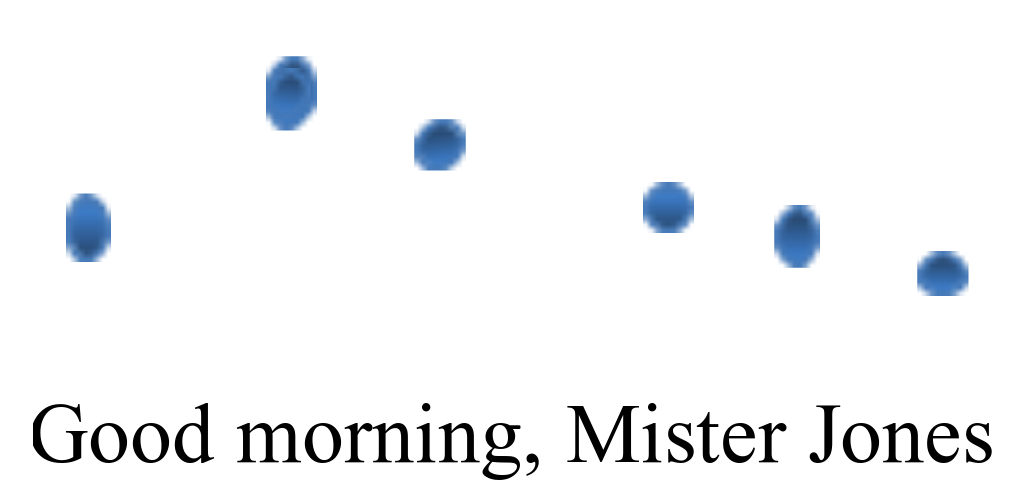
\includegraphics[width=0.5\textwidth]{figures/kuiper2_big.png}
\caption{Primary school greeting formula tune.}
\label{fig:05:02}
\end{figure}


\il{M\=aori}
\ea\label{ex:ex08}
M\=aori\\
\gll Tihei   mauri ora\\
  sneeze spirit  life\\
\glt ‘the sneeze of life’
\z


\pref{ex:ex08} is used by a speaker when taking the floor during Maori oratory.

The formula has an intonationally raised and prosodically drawn out syllable on \textit{hei} and a quicker than normal downward intonation contour on the remaining syllables of the phrase. This is also a Type~1 idiosyncrasy since such intonation contours are possible within the grammar. \is{intonation}

Any lexical item may have conventional conditions of use such as \pref{ex:ex09}--\pref{ex:ex11}. This is a digital Type~1 property since the grammar has nothing to say about the usage conditions of lexical items. Such lexical items are often termed formulae or routine formulae  \citep{Coulmas1979}.

\begin{exe}
\ex\label{ex:ex09} Sorry.
\end{exe}

\noindent
a single word apology,

\begin{exe}
\ex\label{ex:ex10} Bullshit!
\end{exe}

\noindent
a compound word exclamation of disbelief,

\begin{exe}
\ex\label{ex:ex11} If it please Your Honour.
\end{exe}

\noindent
an MWE used by legal counsel seeking approval for a course of action of a presiding judge in a court

\il{M\=aori}
An example from M\=aori is the formula in \pref{ex:ex12}. 


\begin{exe}
\ex\label{ex:ex12} kapiti hono,       t\=atai   hono\\
‘join   connect,  recite connect’
\end{exe}

\noindent
This is a bridging formula used to transition from the acknowledgement of the dead to greetings to the living in formal speechmaking.

While %we 
I have designated this property as digital, i.e. an MWE either does or does not have specific 
conditions of use, the specific conditions of use are themselves complex and not necessarily 
digital \citep{Biber1994}. The contexts of use will also range from the general to the specific. 

\subsection{Idiosyncratic properties MWEs may have by virtue of their being structurally complex}

Such properties are shared by structurally complex words.

It is possible for a MWE to exhibit morphological and/or morpho-syntactic idiosyncrasy. The extent to which this is possible depends on the inflectional and derivational morphology of a language.\footnote{   Note that it is rare for left hand constituents of \il{English} English compounds to have inflections even when this is warranted semantically as in \textit{head count} ‘the counting of heads’. This restriction on the appearance of inflections appears to be a requirement of the word formation rules of English and thus not an idiosyncratic property of individual compounds.}  Languages with extensive inflectional morphology such as Turkish \il{Turkish} would be expected to exhibit inflectional idiosyncrasy in their MWEs. Chinese languages in the absence of inflectional morphology cannot. For example, in English an MWE may have an obligatory singular when a plural is semantically plausible as in \pref{ex:ex13} or an obligatory plural as in \pref{ex:ex14} when a singular is plausible. These are Type~1 idiosyncrasies.

\begin{exe}
\ex\label{ex:ex13}   give someone a hand\\
‘assist someone’\\
\#give someone a pair of hands
%\end{exe}

%\begin{exe}
\ex\label{ex:ex14}  as scarce as hens’ teeth\\
  ‘very scarce’\\
  \#as scare as a hen’s teeth
\end{exe}

MWEs may also have idiosyncratic derivational morphology. In the MWE in \pref{ex:ex15},

\begin{exe}
\ex\label{ex:ex15}   the use of undue force\\ 
or: to use undue force
\end{exe}

\noindent
this formula is used of police arrests in particular. The morphological idiosyncrasy is that there is no equivalent with \textit{due force} (although there are no doubt situations where due force is applied). 

%\marginpar{I transformed this into a sentence. Please check!}
In M\=aori, the expression \il{M\=aori}


\ea\label{ex:ex16}
\gll m\=a-na    (noa ake) te     kore e        V (o NP)\\
     \textsc{prep}.\textsc{3sg} (just up)  \textsc{det} \textsc{neg} \textsc{tam} V (\textsc{prep} NP)\\
\glt Lit. (His/they, \ldots) not Ving~is (just) his fault.
\glt ‘NP is certain to V’
\z

\noindent
occurs in the 
example sentence in \pref{ex:ex16b}.
%\begin{exe}
\ea\label{ex:ex16b}
\gll %\sn 
M\=ana      noa ake te     kore e         pai    o  t\=a     t\=atou        r\=arangi\\
\textsc{prep}.\textsc{3.sg}  just up  \textsc{det} \textsc{neg} \textsc{tam}  good of \textsc{sg.A} \textsc{l.pl.inc}  line\\
\glt ‘Just because of him our lineout was no good.’%
\footnote{Detailed glosses: 
\textit{M\=ana} 'for him/her'; 
\textit{noa ake} 'just/merely'; 
\textit{t\=a t\=atou =} 'ours (first person inclusive)', i.e., 'belonging to all of us'.
}
\z

%\end{exe}
%‘Just because of him our lineout was no good.’%
%\footnote{http://www.nzherald.co.nz/nz/news/article.cfm?c\_id=1\&objectid=10587508}
%\end{exe}

\noindent
This is from a piece of talk about rugby football in which lineouts are a set move.%
\footnote{Source: http://www.nzherald.co.nz/nz/news/article.cfm?c\_id=1\&objectid=10587508.}

%http://www.nzherald.co.nz/nz/news/article.cfm?c\_id=1\&objectid=10587508

This MWE has the restriction that it always contains \textit{m\=ana}, with 3\textsuperscript{rd} person singular agreement, whatever the number of the subject NP. This is a case where the VP has a frozen morphology and agreement does not operate across the boundary between the open slot of the subject and the number inflection of the verb. Since the general rules of agreement do not operate in this case, this is a Type~2 idiosyncrasy.

An MWE may also retain as an idiosyncratic property an inflection which is no longer available in the current language. The Dutch MWE in \pref{ex:ex17} \il{Dutch}

%\begin{exe}
\ea
\label{ex:ex17}\gll des duivels\\
     the.\textsc{gen} devil.\textsc{gen}\\
\glt ‘to be very angry’ 
\z
%\end{exe}

\noindent
exhibits a genitive inflection \is{genitive} on the article which is no longer current. This is a Type~2 idiosyncrasy since \pref{ex:ex17} exhibits a breach of the current rules of inflection.

It is also possible that an individual word may have different \is{morphosyntax} morphosyntactic properties in an MWE than it does elsewhere.  An anonymous reviewer has given the following example from French. ‘To cite from Grevisse (Bon Usage: 198) “\textit{Orge} est féminin, sauf dans les deux expressions \textit{orge mondé}, \textit{orge perlé.}” So a word may be feminine, except in certain fixed expressions.’ Here presumably agreement with the gender of the noun would be un-idiosyncratic. This is a Type~1 idiosyncrasy since the grammar of French \il{French} makes three genders available and the assignment of gender to individual words is (in part) arbitrary.

All structurally complex lexical items can have bound forms as constituents, derived words such as \textit{a}\textbf{\textit{gog}}\textit{,} c.f.\@ \textit{adrift}, compound words such as \textbf{\textit{ward}}\textit{robe} \citep{Richter2010}. In MWEs the following examples show the presence of bound words:%
\footnote{In \pref{ex:ex18}, \textit{h\=onia} is a bound form occurring only as a modifier of \textit{m\=angere} ‘lazy’.}  

\il{M\=aori}
\begin{exe}
\ex\label{ex:ex18}    M\=aori\\ 
\gll m\=angere \textbf{\textit{h\=onia}} \\
                      lazy     very\\
                      \glt 'very lazy'
%\end{exe}


%\textit{h\=onia} is a bound form occurring only as a modifier of \textit{m\=angere} ‘lazy’.  

%\begin{exe}
\ex\label{ex:ex19}  be on \textbf{tenterhooks}\\
  ‘to be in a state of agitation about a future event’
%\end{exe}


%\begin{exe}
\ex\label{ex:ex20}   take \textbf{umbrage} at\\
 ‘take offence at’
%\end{exe}

%\begin{exe}
\ex\label{ex:ex21}    \textbf{kith} and kin\\
  ‘relatives’
\end{exe}



Being a bound word is a Type~1 idiosyncrasy since no rule of the grammar is breached by the fact that a word is bound within an MWE.

\bigskip
While this chapter will not specifically deal with the semantic idiosyncrasy of MWEs, it is useful to offer a few remarks on that property since it is shared with structurally complex lexical items such as derived and compound words. Semantic idiosyncrasy appears to be an analogue 
property.%
\footnote{See \citet{Burger2010} for a useful introductory discussion.} 
%
Semantic idiosyncrasy can come about in a number of ways. As 
\citet{Jackendoff1975} points out, many \il{English} English derivational affixes are 
polysemous. In particular words, however, only one of the senses 
associated with the affix is part of the compositional reading of the word 
as a whole. Such selective compositionality occurs where not all the 
cross-product senses of affixes or words are part of the sense of the 
whole expression. In an MWE such as \pref{ex:ex22},

\begin{exe}
\ex\label{ex:ex22}    BE in stock\\
  ‘be part of the current inventory of a shop or warehouse’
\end{exe}

\noindent
the word \textit{stock} does not have the sense of ‘liquid used for soups and sauces’ but  ‘inventory’.\footnote{   This selective compositionality may be the consequence of polysemy or homonymy. It can be difficult to separate these in particular instances.} This is a Type~1 idiosyncrasy since such a reading is a possible reading but not the only possible one.

Non-compositionality can occur where the sense of a word in a lexical item 
does not occur when the word is used independently. This is not a matter 
of a breach of a grammatical or semantic rule. It would therefore be a 
Type~1 idiosyncrasy. It is manifest in a MWE such as \pref{ex:ex23}.

\begin{exe}
\ex\label{ex:ex23}     without let or hindrance\\
‘without any obstruction or interruption’
\end{exe}

\noindent
The noun \textit{let} has a now defunct syntactic category and sense.%
\footnote{It also has this sense in the term \textit{let} in tennis, namely an obstruction.}

A second kind of non-compositionality occurs when the rules of the semantics of the language are breached as in conventional figurative expressions such as \pref{ex:ex24}. These are Type~2 idiosyncrasies. In such cases structurally complex lexical items also share the potential property of having analysable semantic representations. In \pref{ex:ex24}, the phrase is figurative with the gloss ‘accepting a difficult challenge or situation’, \textit{grasp} being ‘accept’ and the \textit{nettle} being ‘the difficult challenge or situation’.

\begin{exe}
\ex\label{ex:ex24}    grasp the nettle
\end{exe}



\section{Idiosyncratic structural properties a MWE may have by virtue of being a phrase}

In this section, % we 
I focus on those areas of potential structural idiosyncrasy which MWEs have but which they do not 
share with other structurally complex lexical items such as derived and compound words. Each 
relevant area will show that the Law of Exceptions appears to be corroborated. \is{Law of Exceptions}


All MWEs are associated with a phrase structural configuration. This is shown for one MWE in example \pref{ex:ex25}, where the final NP is a slot (an open argument position).

\begin{exe}
\ex\label{ex:ex25}   [VP[V \textit{make}][NP[DET \textit{the}][N \textit{most}][PP[P \textit{of}][NP]]] \\
‘maximize the potential offered by \ldots’ 
\end{exe}


Having grammatical structure is a digital property. That is not 
to say that such structures are always permissible in the 
current synchronic grammar of the language as in
\pref{ex:ex26}.

\begin{exe}
\ex\label{ex:ex26} be that as it may\\
‘whatever the actual case may be’
\end{exe}


Example \pref{ex:ex26} is in the subjunctive mood, a mood that no longer exists in the current synchronic grammar of \il{English} English.\footnote{ This is essentially a morpho-syntactic property included here as a structural property.} This is a Type~2 idiosyncrasy.

In \pref{ex:ex27}, the syntax is calqued from a Chinese four character idiom \citep{rohtua}.\il{Chinese}

\begin{exe}
\ex\label{ex:ex27} long time no see\\
‘I haven’t seen you for some time’ 
\end{exe}

\noindent
 It can therefore be concluded that there are exceptions to the phrase structural regularities of the synchronic grammar. This is also a Type~2 idiosyncrasy. 

The phrase structure of MWEs may be further constrained by general constraints that are lexicon internal in that not all the possible phrase structural configurations the grammar allows are to be found in MWEs. For example, grammars allow for recursive rules in their syntax. There is evidence of a degree of recursion in MWE as in \pref{ex:ex28}.

\begin{exe}
\ex\label{ex:ex28} a sight for sore eyes\\
‘a welcome appearance’ 
\end{exe}



In \pref{ex:ex28}, there are two NPs one is the top NP while the other is embedded in a PP. However recursion is limited because MWEs are stored in a finite brain and so cannot be of indefinite length. How limited recursion in MWEs may be is an open question.\footnote{   Hoeksema, and Richter \& Sailer (this volume) discuss MWEs of clause length.} The Law of Exceptions \is{Law of Exceptions}is, however, corroborated as regards recursion in the grammar since this is a Type~2 idiosyncrasy albeit a general one since it is not just the property of a single lexical item.

\citet{OGrady:98} proposes that the citation form of idioms in the mental lexicon is in the form of lexical selection by heads of heads within their syntactic domains thus forming chains of heads. Some of these requirements are interesting in that, while phrases must have heads, it is not a necessary property of MWEs that the head position should dominate a lexical item or, in the case of functional projections, a specific functional head. This constraint may itself have exceptions, as suggested by an example from M\=aori as in \pref{ex:ex29}, \il{M\=aori}
a formula expressing sympathy for someone's problem.

\begin{exe}
\ex\label{ex:ex29} 
\gll i     w\=ana       nei         (hoki)\\
  at/by/from   his/her     \textsc{near-speaker} \textsc{emphatic-particle}\\
  %emphatic particle
\end{exe}



While \textit{i} is the head of the PP, O’Grady’s theory predicts that there must be a lexical head for \textit{i} to select within the immediate domain of the PP, i.e. the head of the NP complement of \textit{i}. \textit{Hoki} is not a lexical head and is optional (therefore cannot be a lexical head).  \textit{W\=ana} ‘his/her’~can be replaced by an appropriate possessive determiner, eg. \textit{w\=au} ‘your’, \textit{w\=a r\=atou} ‘their’. There are however restrictions on the choice of possessives. The possessive pronoun always starts with \textit{w}, a possible initial phoneme for these possessives otherwise, but many speakers use it only here. Normally the possessive determiners have \textit{t-} for singular possessum,~Ø- for plural, thus eg \textit{t\=ana} {\textasciitilde}\textit{\=ana}. Some speakers allow \textit{w-}, thus \textit{w\=ana} for plural. However all speakers use only the \textit{w-}forms in this MWE showing an idiosyncrasy typically associated with MWEs.~ Furthermore the possessive (taking possessive to be determiners) has no NP complement. The determiner position is also always a possessive, i.e., \textit{i w\=ona nei} 
can not occur in this MWE. \textit{I w\=ona nei} can certainly appear elsewhere given the right syntactic etc environment as in \pref{ex:ex30}; just never in this MWE.

\ea\label{ex:ex30}
\gll He nui ake     \=oku waka i    w\=ona nei.\\
                    A  big upwards my    cars than his    here'\\
\glt 'My cars are bigger than his.'
\z


\textit{Nei} is obligatory. While in the morpho-syntax of M\=aori \il{M\=aori} there are three locative particles, one never finds either of the other locative particles: \textit{n\=a}, ‘near hearer’ or \textit{r\=a} ‘over there’ in this MWE. So there are no lexical heads within the domain of the head position of this MWE and the non-heads are idiosyncratic in various ways. Thus, unless one~uses an analysis allowing functional heads to serve in O’Grady’s head chain proposal in which \textit{w\=ana} etc. are~Determiners and thus functional heads, this MWE has no lexical head within the immediate domain of the head of the MWE.\footnote{   Ray Harlow (personal communication) provided this example and analysis. A case might be made for functional heads as well as lexical heads being predicted to be lexicalized in the case of possessives where the possessive marker could be regarded as a functional head of DP and where the NP within the possessive phrase is a slot.} This case therefore suggests that a strong form of O’Grady’s proposal is falsified and the Law of Exceptions is corroborated. \is{Law of Exceptions}

The syntax of a language may require certain obligatory constituents, e.g. 
complements of transitive verbs or possessive NPs. In an MWE these may not 
be filled with lexicalized material as in \pref{ex:ex31} and 
\pref{ex:ex32}. Where this is the case the idiosyncrasy is lexical and is 
not a breach of the rules of the syntax. It is an idiosyncrasy because, 
while \textit{take} is transitive, it is an idiosyncratic feature of the 
MWE that the NP object of \textit{take} in \textit{take NP to task} is not 
lexically filled as it is in \textit{take notice of}. 
Thus these are Type~1 idiosyncrasies.

\begin{exe}
\ex\label{ex:ex31} take NP to task\\
‘hold someone responsible’
%\end{exe}



%\begin{exe}
\ex\label{ex:ex32} get NP’s goat.\\
‘annoy someone’
\end{exe}



Such slots may be semantically restricted in idiosyncratic ways as in \pref{ex:ex33}.

\begin{exe}
\ex\label{ex:ex33} drop in on NP[+human]\\
‘visit someone unannounced’
\end{exe}



Some MWEs have an optional but lexicalized constituent as in \pref{ex:ex34}. Again this does not involve a syntactic irregularity since the rules of the syntax allow both configurations. In other words, while \textit{drop} can have both human and non-human objects, \textit{drop in on} can only have a human object. So these are also Type~1 idiosyncrasies.

\begin{exe}
\ex\label{ex:ex34} (keep poss{}-NP) fingers crossed\\
‘hope for a good outcome’
\end{exe}



Such optional constituents are either truncations \is{truncation} as in \pref{ex:ex33} or they can be internal to the MWE as in \pref{ex:ex35}.

\begin{exe}
\ex\label{ex:ex35}  take (careful) note of NP
\end{exe}

In \pref{ex:ex35}, \textit{careful} is a highly preferred modifier and thus we can suppose that it is lexicalized but optional. Given that modifiers are permissible in general, this is a Type~1 idiosyncrasy.

The distinction between slots and optional constituents is that slots are lexically unspecified except for their syntactic category and are obligatory, optional constituents are lexically specified and optional while modifiable MWEs are optionally able to take any appropriate modifier.

Conversely, in some MWEs, internal modification having scope over an internal constituent is not permitted, for example in the case of \pref{ex:ex36}.

\begin{exe}
\ex\label{ex:ex36} cut no ice\\
‘have no impact’
\end{exe}



This cannot be modified, as shown in \pref{ex:ex37},

\begin{exe}
\ex\label{ex:ex37} \#cut no melting ice
\end{exe}

\noindent
when the grammar would otherwise permit it.%
\footnote{   The semantics of modifier constituents within MWEs is complex \citep{Nicolas1995}. Nicolas suggests that a modifier 
placed internally to a MWE can have scope over the meaning of the whole 
expression. In \pref{ex:ex35} the internal modifier \textit{melting} 
cannot be parsed as modifying \textit{ice}. However there are other cases 
Nicolas regards essentially as adverbial in having scope over the 
metaphorical expression as a whole so that \textit{cut no real ice} is 
parsed as  'really cut no ice' and \textit{cut no empirical ice} is parsed 
as\textit{} 'cut no ice empirically'. So the modification, while placed 
internally, is not semantically a modification of the constituent the 
modifier is predicted to modify in a compositional syntax. These cases are 
thus idiosyncratic. In that sense the placement of the modifier is 
structurally idiosyncratic.} 
This suggests that modifiability properties 
can sometimes be absolute such as cases where modifiability is impossible 
whereas for other MWEs it may be a preferred option with some highly 
favoured and other disfavoured modifiers. 

The presence of a lexicalized optional modifier in \pref{ex:ex35} is idiosyncratic but it is not a grammatical irregularity. It is therefore a Type~1 idiosyncrasy. The restriction against modification in \pref{ex:ex36} could, by contrast, be regarded as a grammatical irregularity, i.e. a Type~2 idiosyncrasy. That such cases should exist is a prediction of the Law of Exceptions. \is{Law of Exceptions}

Where the syntax of a language allows a variety of related constructions for a similar argument structure, an MWE may only permit one or fewer than a full set of variations, e.g. double object constructions as in \pref{ex:ex38}--\pref{ex:ex41}, passives as in \pref{ex:ex42} and \pref{ex:ex43}. This is a Type~1 idiosyncrasy.

\begin{exe}
\ex\label{ex:ex38} give NP the sack\\
‘terminate NP’s employment’
%\end{exe}

%\begin{exe}
\ex\label{ex:ex39} \#give the sack to NP.
%\end{exe}

%\begin{exe}
\ex\label{ex:ex40} \#pay something attention
%\end{exe}

%\begin{exe}
\ex\label{ex:ex41} pay attention to something\\
‘note or concentrate on something’
%\end{exe}

%\begin{exe}
\ex\label{ex:ex42} NP cut off his/her nose to spite his/her face\\
‘act in a way that is detrimental to oneself out of pique’
%\end{exe}

%\begin{exe}
\ex\label{ex:ex43} \#John’s nose was cut off to spite his face.
\end{exe}

For each set of syntactic alternates of this kind there may be MWEs which are idiosyncratic in allowing only one of the two possibilities where the grammar would predict that both might occur. For example, a double object construction may be lexicalized in either one or other form as in \pref{ex:ex38}--\pref{ex:ex41}, or both as in \pref{ex:ex44} and \pref{ex:ex45}.

\begin{exe}
\ex\label{ex:ex44} give credit to NP (for)\\
‘give positive acknowledgement to someone for something’
%\end{exe}

%\begin{exe}
\ex\label{ex:ex45} give NP credit (for)
\end{exe}

\noindent
Such distributions may well be matters of degree.\footnote{   \citet{Fraser1970} hypothesises that there is a hierarchy of frozenness in construction types while \citet{Nunberg1994} propose that the degree of syntactic flexibility is related to the degree of compositionality of the MWE.} 

In an MWE the antecedent of a pronominal or reflexive can be more restricted than the syntax of a language requires. Such cases can be seen as slots which are restricted to pronominals with additional slot restrictions as regards the antecedent of the pronominal. This is a Type~1 idiosyncrasy.

In \pref{ex:ex46}, the antecedent of the possessive must be the agent argument of \textit{dig} as in \pref{ex:ex47} and \pref{ex:ex48}.

\begin{exe}
\ex\label{ex:ex46} dig one's heels in\\
%dig poss-PRON heels in\\
‘resist’ 
%\end{exe}
\begin{xlist}
%\begin{exe}
\ex\label{ex:ex47} Jane dug her heels in,
%\end{exe}

%\begin{exe}
\ex\label{ex:ex48} \#Jane dug Fred’s heels in.
\end{xlist}
\end{exe}

An MWE can have argument structure which is different from that of its head verb as in \pref{ex:ex49}. This again a Type~1 idiosyncrasy since the grammar allows for predicates to have various argument structures.

\begin{exe}
\ex\label{ex:ex49} raining cats and dogs\\
‘raining heavily’
\end{exe}

\noindent
\textit{Rain} is a zero place predicate but in \pref{ex:ex49} it is 
apparently a one place predicate.%
\footnote{   This could be seen as a case of a lexicalised internal accusative such as one gets with \textit{It snowed a blizzard}.}  

MWEs merge into the constructions of Construction Grammar. They are of two kinds: lexically motivated constructions, e.g. the \textit{let alone} construction \citep{FillmoreEtAl1988}, and syntactically motivated constructions, e.g. irreversible binomials \citep{Malkiel1959}. It is an open question whether the later belong in the phrasal lexicon or in the grammar. The former clearly do belong in the lexicon given that they have lexical content.

As suggested above, the grammars of languages place limits on phraseological variation. Typologically different languages will therefore be predicted to give different ranges of idiosyncrasies for MWEs. One typological distinction, is that between what are termed free word order languages but are more accurately free phrase order languages such as Warlpiri \il{Warlpiri} and Latin.\footnote{   Ray Harlow (personal communication) indicates that no dictionary of \il{Latin} phraseological units exists for Latin and Michael Walsh (personal communication) knows of no dictionaries of phrasal vocabulary for any aboriginal language.}  Questions which are yet to be answered about such languages is what the underlying form of the syntactic representation of the MWEs of such languages might be. How flexible are their MWEs given that the languages themselves have relatively free phrase order? In turn what idiosyncrasies might their MWEs display in the relevant areas of the grammar?\footnote{   Michael Walsh and Maia Ponsonnet (personal communication) know of no studies that might assist in answering these questions.}

\il{Dutch}
What of languages with the typological character of so called verb second (V2) languages such as Dutch and German where the canonical order, within a generative framework, in main clauses is I second but in subordinate clauses I last? German and Dutch phrasal dictionaries list VP idioms with the verb in VP final position although in main clauses the tensed verb will be in second position. For example, a Dutch MWE as in in \pref{ex:ex50} is verb last in subordinate clauses as in \pref{ex:ex51} but verb second as in \pref{ex:ex52}.

\ea\label{ex:ex50}
\gll \textbf{van} NP \textbf{houden}\\
             from someone/something hold\\
\glt ‘love someone/something’
\z


\ea\label{ex:ex51}
\gll   Ik  dacht    dat  ik \textbf{van} mijn aapje houden  wou. \\
I   thought that I  from my  {little monkey} hold      would. \\
\glt ‘I though that I would love my little monkey’
\z

\ea\label{ex:ex52}
\gll Ik \textbf{hielt} \textbf{van} mijn aapje,\\
I  held  from my  {little monkey}\\
\glt ‘I loved my little monkey’. 
\z

Verb second placement is also obligatory if the verb is the head of a VP MWE.\footnote{    This phenomenon is also discussed by \citet{Schenk:95}, \citet{Nunberg1994} and Bargmann \& Sailer (this volume).}


\ea\label{ex:ex53}
\gll Ik dacht  dat  ik het gewoon \textbf{uit}   \textbf{mijn} \textbf{duim}   \textbf{zuigen} kon.\\
  I  thought that I   it    just       out     my   thumb suck    could\\
\glt  ‘I though I could just make it up.’
\z

\ea\label{ex:ex54}
\gll Ik \textbf{zoog} het gewoon \textbf{uit}     \textbf{mijn}  \textbf{duim}.\\
  I  sucked  it    just       out      my   thumb\\
\glt  ‘I just made it up.’
\z

\il{Dutch}\il{German}
What is the order in German and Dutch of the verb plus its complement for such MWEs in the mental lexicon? Is there an order at all or are there only dependencies? This not a question of flexibility under movement. Verb second placement in main clauses is obligatory. Are there Type~2 idiosyncratic manifestations of these regularities in the MWEs of German and Dutch? The Law of Exceptions predicts that there should be cases in Dutch and German of MWEs which have main clauses where the tensed verb is not in second position.

Beyond the Law of Exceptions \is{Law of Exceptions} lies a further question as to the preponderance in the lexicon of a language of particular classes of exceptions. 
It is possible that different languages make different selective use of the parameters of variation noted above, e.g. some languages might have 
more bound words than others \citep{Dobrovolskij1988}.

\section{Conclusion}

The foregoing provides an outline of a set of structural properties of a grammar which have the potential to have exceptions and thus give rise to idiosyncratic structural properties of MWEs. It has been proposed that such exceptions are of two kinds: those which are ‘basic irregularities’, i.e. which are in breach of the rules of the grammar and which %we 
I have termed Type~2 idiosyncrasies, and idiosyncrasies which are the result of arbitrary restrictions on lexical items where the grammar makes no stipulation about such restrictions. Where such idiosyncrasies appear in lexical items, these have been termed Type~1 idiosyncrasies. By classifying idiosyncrasies on the basis %we 
I have, it also seems that Type~1 idiosyncrasies may be more common and diverse than Type~2 idiosyncrasies and that the lexicon is not as full of seriously lawless inmates as the prison metaphor in \citet{DiSciullo1987} suggests. Perhaps there is a maximum security wing for Type~2 inmates and a less secure set of cell blocks for Type~1 inmates whose deviance is by way of arbitrary restriction. 

\section*{Acknowledgements}

My considerably thanks to the editors of this chapter 
and its anonymous reviewers for numerous corrections and suggestions.  I 
am grateful to Ray Harlow for the M\=aori examples. Note there has been no 
systematic study of the phraseology of M\=aori.





{\sloppy
\printbibliography[heading=subbibliography,notkeyword=this]
}
\end{document}
